\begin{table}
\begin{center}
\begin{tabular}[H]{|l|}
\hline
\multicolumn{1}{|c|}{\textsc{T6}}\\
\hline
\begin{tabular}{c|l}
\begin{minipage}{85mm}
\vspace{2mm}
\begin{center}
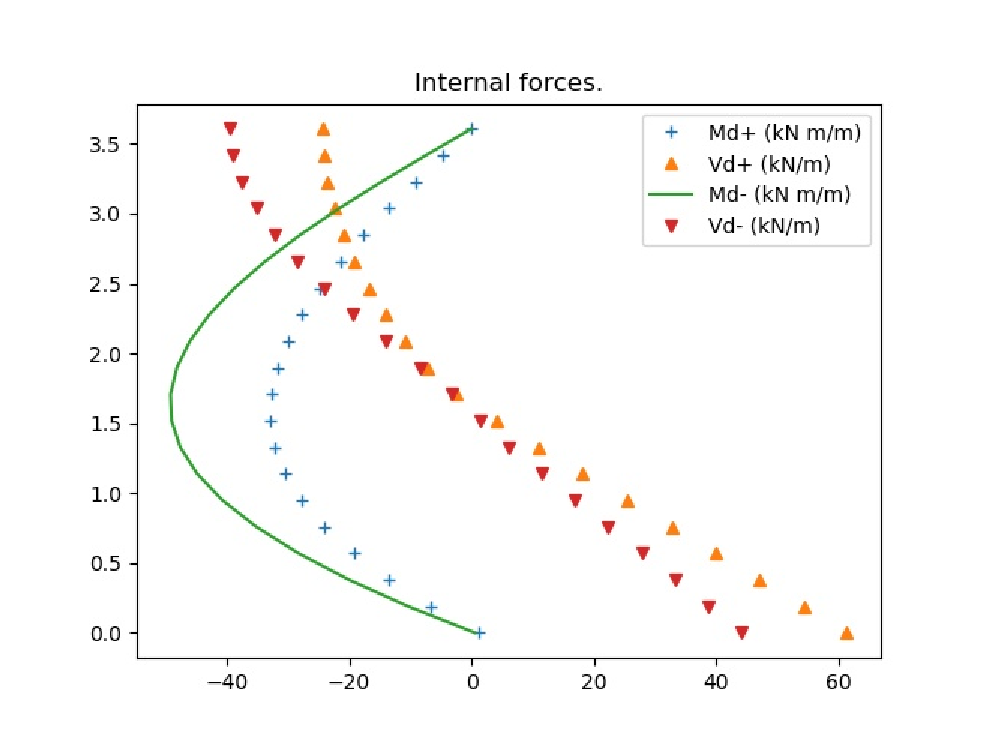
\includegraphics[width=80mm]{T6}
\end{center}
\vspace{1pt}
\end{minipage} & 
\begin{tabular}{l}
\textsc{Wall geometry}\\
Stem top thickness: \\
$b_{top}= 0.25\ m$\\
Stem height: \\
$h_{stem}= 3.43\ m$\\
Stem bottom thickness: \\
$b_{bottom}= 0.25\ m$\\
Footing thickness: \\
$b_{footing}= 0.36\ m$\\
\end{tabular} \\
\end{tabular} \\
\hline
\begin{tabular}{llll}
\multicolumn{3}{c}{\textsc{Materials}}\\
  Concrete: C4000 &   Steel: A615G60 &   Concrete cover: 55 mm\\
\end{tabular} \\
\hline
\end{tabular}
\caption{Wall materials and dimensions T6} \label{tb_def_T6}
\end{center}
\end{table}
\begin{center}
\begin{tabular}[H]{|l|c|c|c|}
\hline
\multicolumn{4}{|c|}{\textsc{wall: T6 stability check}}\\
\hline
Vérification:  & $F_{disp}$ & $F_{req}$ & Combination\\
\hline
Overturning:  & 13.59 & 1.00 & EQ1609A\\
Sliding:  & 1.10 & 1.00 & EQ1609A\\
Bearign capacity:  & 0.43 & 1.00 & EQ1609A\\
Adm. pressure:  & 1.03 & 1.00 & EQ1613B\\
\hline
\multicolumn{4}{|l|}{$F_{avail.}$: available security.}\\
\multicolumn{4}{|l|}{$F_{req}$: required security.}\\
\hline
\end{tabular}
\end{center}
\begin{center}
\begin{tabular}[H]{|l|c|c|c|}
\hline
\multicolumn{3}{|c|}{\textsc{Wall: T6 rotation check}}\\
\hline
$\beta_{disp} (\permil)$ & $\beta_{req}(\permil)$ & Combination\\
\hline
-1.37 & 2.00 & ELS00\\
\hline
\multicolumn{3}{|l|}{$\beta_{disp}$: wall maximum computed rotation.}\\
\multicolumn{3}{|l|}{$\beta_{req}$: wall maximum admissible rotation.}\\
\hline
\end{tabular}
\end{center}
\bottomcaption{T6 wall reinforcement} \label{tb_T6}
\tablefirsthead{\hline
\multicolumn{1}{|c|}{\textsc{Reinforcements mur T6}}\\\hline
}
\tablehead{\hline
\multicolumn{1}{|c|}{\textsc{T6 (suite)}}\\\hline
}
\tabletail{\hline \multicolumn{1}{|r|}{../..}\\\hline}
\tablelasttail{\hline}
\begin{center}
\begin{supertabular}[H]{|l|}
\hline
\textbf{Reinforcement 1 (outside reinforcement dowels) :} \\
  RC section dimensions; b= 1.00 m, h= 0.25 m\\
  diam: 16 mm, spacing: 300 mm  reinf. development L=0.34 m (22 diameters).\\
  diam: 19 mm, spacing: 300 mm  reinf. development L=0.61 m (32 diameters).\\
  area: As=  16.13 cm2/m areaMin:   4.56 cm2/m  F(As)= 3.54 OK!\\
  Bending check: Md=   7.38 kN m, MR=  99.62kN m  F(M)= 13.49 OK!\\
  Shear check: Vd=  51.43 kN,  VR= 199.37 kN  F(V)= 3.88 OK!\\
  Stress check: M=   7.38 kN m, $\sigma_s$=  20.02 MPa\\
    $\sigma_{lim}$= 230.00 MPa  F($\sigma_s$)= 11.49 OK!\\
\textbf{Reinforcement 3 (footing top reinforcement):}\\
  RC section dimensions; b= 1.00 m, h= 0.36 m\\
  diam: 16 mm, spacing: 300 mm  reinf. development L=0.34 m (22 diameters).\\
  diam: 19 mm, spacing: 300 mm  reinf. development L=0.61 m (32 diameters).\\
  area: As=  16.13 cm2/m areaMin:   6.38 cm2/m  F(As)= 2.53 OK!\\
  Bending check: Md=   1.65 kN m, MR= 152.86kN m  F(M)= 92.67 OK!\\
  Shear check: Vd=   2.01 kN,  VR= 279.12 kN  F(V)= 138.73 OK!\\
  Stress check: M=   1.65 kN m, $\sigma_s$=   3.19 MPa\\
    $\sigma_{lim}$= 230.00 MPa  F($\sigma_s$)= 71.99 OK!\\
\textbf{Reinforcement 4 (inside reinforcement dowels):}\\
  diam: 10 mm, spacing: 150 mm  reinf. development L=0.30 m (32 diameters).\\
  area: As=   4.73 cm2/m areaMin:   1.72 cm2/m  F(As)= 2.75 OK!\\
\textbf{Reinforcement 5 (inside stem reinforcement):}\\
  RC section dimensions; b= 1.00 m, h= 0.25 m\\
  diam: 19 mm, spacing: 300 mm  reinf. development L=0.61 m (32 diameters).\\
  area: As=   9.47 cm2/m areaMin:   4.56 cm2/m  F(As)= 2.08 OK!\\
  Bending check: Md=  49.02 kN m, MR=  58.26kN m  F(M)= 1.19 OK!\\
  Shear check: Vd=   8.13 kN,  VR= 199.37 kN  F(V)= 24.54 OK!\\
  Stress check: M=  49.02 kN m, $\sigma_s$= 226.52 MPa\\
    $\sigma_{lim}$= 230.00 MPa  F($\sigma_s$)= 1.02 OK!\\
\textbf{Reinforcement 6 (stem top transverse reinforcement):}\\
  RC section dimensions; b= 1.00 m, h= 0.25 m\\
  diam: 13 mm, spacing: 150 mm  reinf. development L=0.30 m (24 diameters).\\
  area: As=   8.60 cm2/m areaMin:   4.56 cm2/m  F(As)= 1.89 OK!\\
\textbf{Reinforcement 7 (footing bottom transverse reinforcement):}\\
  diam: 10 mm, spacing: 150 mm  reinf. development L=0.30 m (32 diameters).\\
  area: As=   4.73 cm2/m areaMin:   3.23 cm2/m  F(As)= 1.47 OK!\\
\textbf{Reinforcement 8 (footing bottom longitudinal reinforcement):}\\
  diam: 16 mm, spacing: 300 mm  reinf. development L=0.34 m (22 diameters).\\
  diam: 19 mm, spacing: 300 mm  reinf. development L=0.61 m (32 diameters).\\
  area: As=  16.13 cm2/m areaMin:   6.38 cm2/m  F(As)= 2.53 OK!\\
\textbf{Reinforcement 9 (footing top longitudinal reinforcement):}\\
  diam: 16 mm, spacing: 300 mm  reinf. development L=0.34 m (22 diameters).\\
  diam: 19 mm, spacing: 300 mm  reinf. development L=0.61 m (32 diameters).\\
  area: As=  16.13 cm2/m areaMin:   6.38 cm2/m  F(As)= 2.53 OK!\\
\textbf{Reinforcement 10 (footing skin reinforcement):}\\
  --\\
\textbf{Reinforcement 11 (stem outside longitudinal reinforcement):}\\
  diam: 13 mm, spacing: 150 mm  reinf. development L=0.30 m (24 diameters).\\
  area: As=   8.60 cm2/m areaMin:   4.56 cm2/m  F(As)= 1.89 OK!\\
\textbf{Reinforcement 12 (stem inside longitudinal reinforcement):}\\
  diam: 13 mm, spacing: 150 mm  reinf. development L=0.30 m (24 diameters).\\
  area: As=   8.60 cm2/m areaMin:   4.56 cm2/m  F(As)= 1.89 OK!\\
\textbf{Reinforcement 13 (stem top skin reinforcement):}\\
  --\\
\hline
\end{supertabular}
\end{center}
